\documentclass[./report.tex]{subfiles}
\usepackage[utf8]{inputenc} % Підтримка UTF-8
\usepackage[ukrainian]{babel} % Підтримка української мови
\usepackage[ukrainian=nohyphenation]{hyphsubst} 
\usepackage{booktabs}
\usepackage[T2A]{fontenc} % Кодова таблиця для кирилиці
\usepackage{amsmath, amsfonts} % Для математики, якщо потрібно
\usepackage[a4paper, left=3cm, right=1.5cm, top=2cm, bottom=2cm]{geometry}
\usepackage{fancyhdr}        % Пакет для налаштування колонтитулів
\usepackage{hyperref}        % Для створення посилань
\usepackage{listings}          % Пакет для вставки коду
\usepackage{graphicx}
\usepackage{csvsimple}
\usepackage{parskip}
\usepackage{csquotes}
\usepackage{pgfplotstable}
\usepackage{xcolor}      % For custom colors

\pagestyle{fancy}            % Встановлюємо fancy стиль для колонтитулів
\fancyhf{}                   % Очищуємо всі колонтитули
% Встановлюємо посилання на зміст у лівий верхній кут
\fancyhead[L]{\hyperlink{mytarget}{Зміст}}  % Посилання на зміст
% Встановлюємо нумерацію сторінок у правий верхній кут
\fancyhead[R]{\thepage}
% Прибираємо колонтитули з першої сторінки
\thispagestyle{plain}
% Прибираємо колонтитули для першої сторінки
\fancypagestyle{plain}{
    \fancyhf{}  % Очищуємо колонтитули
    \renewcommand{\headrulewidth}{0pt}  % Вимикаємо лінію колонтитулів
}
\hypersetup{
    colorlinks=true,        % Enable colored links
    linkcolor=red!50!black,      % Color for internal links
    citecolor=red!50!black,      % Color for citations
    filecolor=red!50!black,      % Color for file links
    urlcolor=red!50!black        % Color for external URLs
}

\graphicspath{{../../../}}

\setlength{\emergencystretch}{3cm}

\usepackage{subfiles}

\begin{document}

\section{ОСНОВНА ЧАСТИНА}
\subsection{Опис даних}
Так як реформа досі продовжується, то дані оновлюються в живому часі.
Тому для дослідження було взято результати \textit{з 25 листопада 2016 по 31 серпня 2024}
\footnote{
  \href{https://data.moenv.gov.tw/en/dataset/detail/aqx_p_488}
  {Покликання на офіційний датасет Міністерства довкілля Тайваню}
}

Відповідно до базового розвідкованого аналізу, було отримано наступні характеристики набору даних:

\begin{itemize}
  \item Кількість рядків: 5\,882\,208
  \item Кількість стовпців: 25
  \item Початковий опис даних:

  \begin{table}[h!]
  \centering
  \begin{tabular}{|>{\raggedright\arraybackslash}p{3cm}|p{5cm}|p{3cm}|}
  \hline
  \textbf{Column} & \textbf{Description} & \textbf{Data Type} \\
  \hline
  date       & Date and time of the reading  & Text    \\
  \hline
  sitename   & Station name                  & Text    \\
  \hline
  county     & County or city                & Text    \\
  \hline
  aqi        & Air Quality Index             & Numeric \\
  \hline
  pollutant  & Main pollutant                & Text    \\
  \hline
  status     & Status of air quality         & Text    \\
  \hline
  so2        & Sulfur Dioxide in ppb         & Numeric \\
  \hline
  co         & Carbon Monoxide in ppm        & Numeric \\
  \hline
  o3         & Ozone in ppb                  & Numeric \\
  \hline
  o3\_8hr    & 8-hour average of Ozone       & Numeric \\
  \hline
  pm10       & Particulate matter under 10m  & Numeric \\
  \hline
  pm2.5      & Particulate matter under 2.5m & Numeric \\
  \hline
  no2        & Nitrogen Dioxide in ppb       & Numeric \\
  \hline
  nox        & Nitrogen Oxides in ppb        & Numeric \\
  \hline
  no         & Nitric Oxide in ppb           & Numeric \\
  \hline
  windspeed  & Wind speed in m/sec           & Numeric \\
  \hline
  winddirec  & Wind direction in degrees     & Numeric \\
  \hline
  unit       & Unit of measurement           & Text    \\
  \hline
  co\_8hr    & 8-hour average of CO          & Numeric \\
  \hline
  pm2.5\_avg & Moving average of PM2.5       & Numeric \\
  \hline
  pm10\_avg  & Moving average of PM10        & Numeric \\
  \hline
  so2\_avg   & Moving average of SO2         & Numeric \\
  \hline
  longitude  & Longitude of the site         & Numeric \\
  \hline
  latitude   & Latitude of the site          & Numeric \\
  \hline
  siteid     & Station ID                    & Numeric \\
  \hline
  \end{tabular}
  \label{tab:data_columns}
  \end{table}
\end{itemize}

\subsection{Підготовка даних}

Для того, щоб розпочати розвідковий аналіз, було проведено очищення та попередня підготовка даних, а саме:

\begin{itemize}
    \item Перший огляд датасету показав, що деякі числові стовпці зчитались як текстові.
    Щоб виправити це, було застосовано функцію `problems` показало, що:

      \begin{itemize}
        \item іноді замість порожнього значення використовується $-$ або ND.
        Через це відповідні колонки стають текстовими
        \item трапляється неправильний формат дати (роздільник $/$ замість очікуваного $-$).
      \end{itemize}

   \textbf{Рішення:} До функції $read\_csv$ додано аргумент $na$, який вказує, що значення
   $" \ "$, $"\ -"$ і $"ND"$ треба сприймати як порожні. Виправлено формат дати.

   Колонки $sitename$, $county$, $pollutant$ і $status$ перетворено на категорійні.
   Проблеми із типами даних на цьому вирішено.

   \newpage

    \item Під час перевірки закодаваних і неадекватних даних у кожному стовпці було отримано наступні результати:
      \begin{itemize}
        \item Стовпці, що містять очевидно кодові значення:
        \begin{itemize}
          \item \textbf{aqi} - кодові: -1
          Рядки, де $\text{aqi} = -1$, майже повністю заповнені NA. Такі рядки займають близько $0.2\%$
          \item \textbf{so2, co, o3, pm10, pm2.5} - кодові: -999

          Є підозрілі від'ємні числа. Можна припустити, що від'ємні показники є наслідком
          неідеалньості калібрування датників (тобто вони є справжніми, а не кодовими).
          Також у датасеті зафіксовані значно більші за модулем додатні концентрації,
          тому зсув показників є незначним.

          \item \textbf{winddirec} - кодові: 990
        \end{itemize}

        \textbf{Рішення:} Кодові значення замінимо на NA.

        \item Стовпці, що містять від'ємні значення:

        \begin{itemize}
          \item \textbf{so2, co, no2,  o3, nox, no, windspeed, co\_8hr, pm2.5\_avg, pm10\_avg , so2\_avg}

          \item \textbf{o3\_8hr} - кодові: -1

          Є від'ємне число -1. Хоча воно і схоже на кодове, за аналогією до попередніх колонок,
          припустимо, що воно справжнє. До того ж, частка таких рядків дуже мала: у цьому можна
          переконатися, поглянувши на гістограму.
        \end{itemize}

        \textbf{Рішення:} Припуститимо, що від'ємні показники є справжніми, а не кодовими, і
        виникли через незначний зсув у калібруванні датників.
        За неохідності (наприклад, для логаритмування) цей зсув можна буде компенсувати
        додаванням певного числа до всіх значень відповідної колонки.

        \item Стовпці, які можна видалити, користь під сумнівом:

        \begin{itemize}
          \item \textbf{unit} - порожня колонка
          \item \textbf{longitude, latitude, siteid} - корисність під сумнівом
        \end{itemize}

        \textbf{Рішення:} Видалимо непотрібні стовпці.
      \end{itemize}

  \item Було перевірено та проаналізовано кількість пропущених значень у кожному рядку та стовпці.
  Відповідно, стовпці в яких було відсутньо більше третини значень, було вирішено видалити,
  а саме в стовпці "pollutant" було відсутньо більше 5%.

  \textbf{Рішення:} видалити стовпець.

  \item Стовпці в яких було відмічено не значний відсоток пропущених даних,
  попередньо було залишено без змін.

  Можливе рішення на майбутнє: заповнити або середніми значеннями (для числового типу),
  або часто повторюваними (для категоріального та текстового)

  \item Було додано додатковий стовпчик з бінарним типом даних: 1 - після реформи, 0 - до реформи.
  Це дозволить проаналізувати та порівняти вплив реформи на якість повітря.
\end{itemize}

В результаті після "очистки" даних, отримали такі основні характеристики:

\begin{enumerate}
  \item Розмір набору даних:
    \begin{itemize}
      \item Кількість рядків: 5\,882\,208
      \item Кількість стовпців: 16
    \end{itemize}
  \item Кількість змінних:
    \begin{itemize}
      \item Факторні (factor) - 3
      \item Логічні (logical) - 1
      \item Числові (numeric) - 11
      \item Тип дати (POSIXct) -  1
    \end{itemize}

  \pagebreak

  \item Кількість пропущених даних:

  \begin{table}[h!]
    \centering
    \begin{tabular}{llccc}
      \hline
      \textbf{Variable Type} & \textbf{Variable} & \textbf{Missing} & \textbf{Complete rate} \\
      \hline
      Factor   & sitename      & 0      & 1     \\
               & county        & 0      & 1     \\
               & status        & 142718 & 0.976 \\
      Logical  & after\_reform & 0      & 1     \\
      Numeric  & aqi           & 50411  & 0.991 \\
               & so2           & 139794 & 0.976 \\
               & co            & 154139 & 0.974 \\
               & o3            & 207427 & 0.965 \\
               & pm10          & 146655 & 0.975 \\
               & pm2.5         & 202228 & 0.966 \\
               & no2           & 166000 & 0.972 \\
               & nox           & 169147 & 0.971 \\
               & no            & 169478 & 0.971 \\
               & windspeed     & 302683 & 0.949 \\
               & winddirec     & 303499 & 0.948 \\
      POSIXct  & date          & 0      & 1     \\
    \end{tabular}

    \caption{Missing data statistics}
    \label{tab:summary}
  \end{table}

  \vspace{1cm}

  \begin{center}
    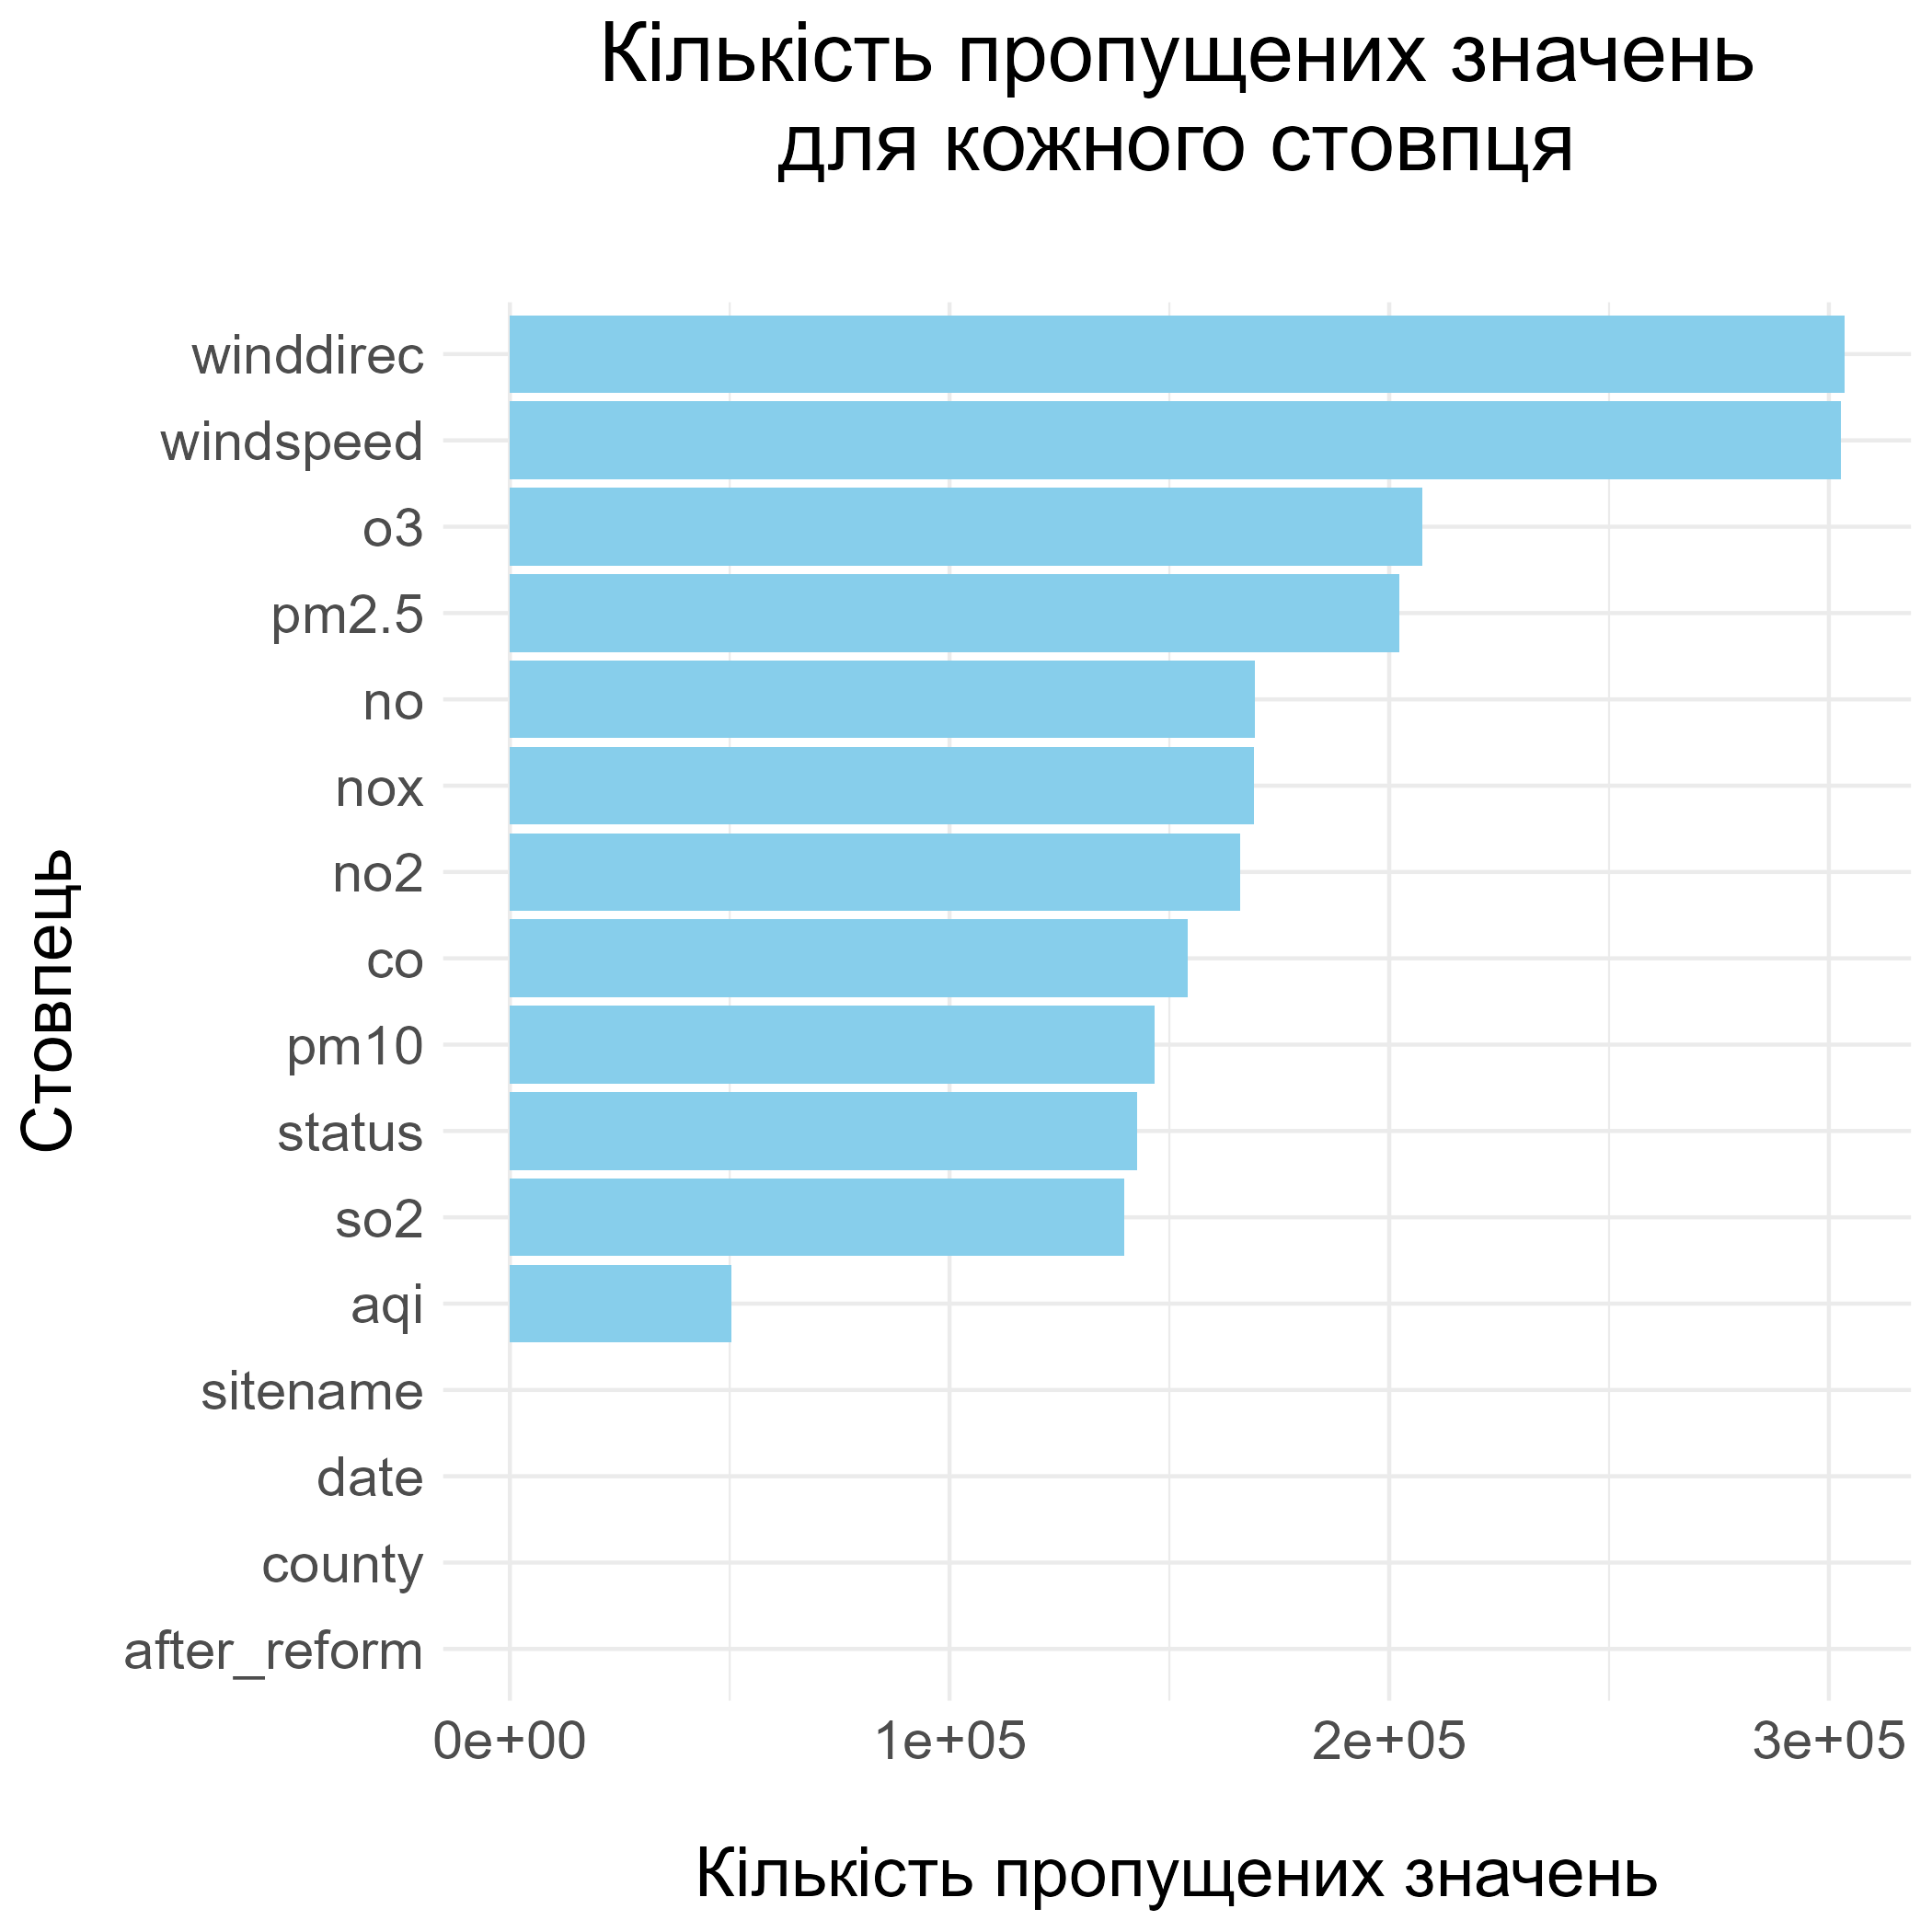
\includegraphics[height=4.5in]{plots/missed_data.png}
  \end{center}

  \pagebreak

  \item Дескриптивнi статистики:

  \begin{itemize}
    \item Числові змінні:

    \begin{tabular}{lcccccc}
    \hline
    \textbf{Variable} & \textbf{Min.} & \textbf{1st Qu.} & \textbf{Median} & \textbf{Mean} & \textbf{3rd Qu.} & \textbf{Max.} \\
    \hline
    aqi       & 0      & 32   & 47    & 54.26 & 70   & 500    \\
    so2       & -4.1   & 1    & 1.7   & 1.99  & 2.5  & 255.4  \\
    co        & -0.27  & 0.19 & 0.29  & 0.34  & 0.41 & 38.58  \\
    o3        & -1     & 16   & 28.3  & 30.42 & 42   & 410    \\
    pm10      & 0      & 18   & 28    & 34.38 & 45   & 1407   \\
    pm2.5     & 0      & 8    & 14    & 16.85 & 23   & 1000   \\
    no2       & -27.78 & 5    & 9     & 11.25 & 15   & 351.05 \\
    nox       & -1.6   & 6.2  & 10.8  & 14.72 & 18   & 431    \\
    no        & -7.2   & 0.7  & 1.4   & 3.45  & 2.7  & 391.31 \\
    windspeed & -0.4   & 1.1  & 1.8   & 2.21  & 2.9  & 41     \\
    winddirec & 0      & 55   & 150   & 163.3 & 270  & 359    \\
    \end{tabular}

    \item Факторні змінні:

    \begin{tabular}{ccccc}
    \hline
    \textbf{Variable} & \multicolumn{4}{c}{\textbf{Count}} \\
    \hline
    status & Good    & Moderate & \vtop{\hbox{\strut Unhealthy for}\hbox{\strut Sensitive Groups}} & Unhealthy \\
           & 3185191 & 2159158  & 343909  & 51008     \\
           & Very Unhealthy  & Hazardous         &                  & \\
           & 173             & 51                &                  & \\
    county & Changhua County & Chiayi City       & Chiayi County    & Hsinchu City  \\
           & 293423          & 71912             & 143986           & 75850         \\
           & Hsinchu County  & Hualien County    & Kaohsiung City   & Keelung City  \\
           & 143846          & 71912             & 888497           & 71913         \\
           & Kinmen County   & Lienchiang County & Miaoli County    & Nantou County \\
           & 71913           & 71914             & 219683           & 216420        \\
           & New Taipei City & Penghu County     & Pingtung County  & Taichung City \\
           & 898819          & 71910             & 305495           & 367033        \\
           & Tainan City     & Taipei City       & Taitung County   & Taoyuan City  \\
           & 366827          & 503766            & 143809           & 448718        \\
           & Yilan County    & Yunlin County     &                  &               \\
           & 147071          & 287491            &                  &               \\
    \end{tabular}

    \item Дата:

    \begin{tabular}{ccc}
      \hline
      \textbf{Variable} & \textbf{Min.} & \textbf{Max.} \\
      \hline
      date & 2016-11-25 & 2024-08-31 \\
           & 13:00:00   & 23:00:00   \\
    \end{tabular}

     \item Логічні:

    \begin{tabular}{ccc}
      \hline
      \textbf{Variable} & \textbf{True} & \textbf{False} \\
      \hline
      after\_reform     &  654783       &  5227425       \\
    \end{tabular}

    \end{itemize}

    \pagebreak

    \item Зменшення набору даних:

    На більшість питань розвідкового аналізу можна дати відповідь не маючи весь набір
    даних. Було прийнято рішення зменшити набір даних, тобто вибрати тільки рядки,
    починаючи з певного року.

    Знайдемо кількість рядків в кожному році:

    \begin{tabular}{cc}
      \hline
      \textbf{Year} & \textbf{Count} \\
      \hline
      2016          & 65431          \\
      2017          & 664415         \\
      2018          & 671559         \\
      2019          & 712824         \\
      2020          & 716022         \\
      2021          & 1070296        \\
      2022          & 748667         \\
      2023          & 736902         \\
      2024          & 496092         \\
    \end{tabular}

    Знайдемо кумулятивну суму з кінця, щоб визначити кількість даних, яка буде вибрана
    починаючи з відповідного року:

    \begin{tabular}{cc}
      \hline
      \textbf{Year} & \textbf{Accumulated count} \\
      \hline
      2016 & 5882208 \\
      2017 & 5816777 \\
      2018 & 5152362 \\
      2019 & 4480803 \\
      2020 & 3767979 \\
      2021 & 3051957 \\
      2022 & 1981661 \\
      2023 & 1232994 \\
      2024 & 496092  \\
    \end{tabular}

    Було прийнято рішення вибрати набір даних починаючи з 2023 року
    (1\,232\,994 з 5\,882\,208 рядків).

    Надалі будемо зазначати на якому наборі даних був виконаний аналіз. Зменшений
    датасет назвемо \textit{trimmed}.

    \item Викиди:

    \quad \textit{Був використаний trimmed набір даних}

    Для пошуку викидів використаємо \textit{фільтр Гампеля}:

    \begin{displayquote}
    Викидом є будь‑яке спостереження
    $x \notin [M - 3 \cdot \text{MAD}; M + 3 \cdot \text{MAD}]$,

    де $\text{MAD} = \dfrac{1}{\Phi^{-1}(0.75)} \cdot \text{median}(\pmb{x} - M)$,
    $M = \text{median}(\pmb{x})$
    \end{displayquote}

    Кількість викидів по кожній змінній:

    \begin{tabular}{ccc}
      \hline
      \textbf{Variable} & \textbf{Count} & \textbf{Relative count} \\
      \hline
      aqi        & 26759  & 0.0217  \\
      so2        & 57595  & 0.0467  \\
      co         & 53340  & 0.0433  \\
      o3         & 5154   & 0.00418 \\
      pm10       & 43393  & 0.0352  \\
      pm2.5      & 43913  & 0.0356  \\
      no2        & 58132  & 0.0471  \\
      nox        & 82640  & 0.067   \\
      no         & 159513 & 0.129   \\
      windspeed  & 43491  & 0.0353  \\
      winddirec  & 0      & 0       \\
    \end{tabular}

   \pagebreak

    Гістограма кількості викидів:

    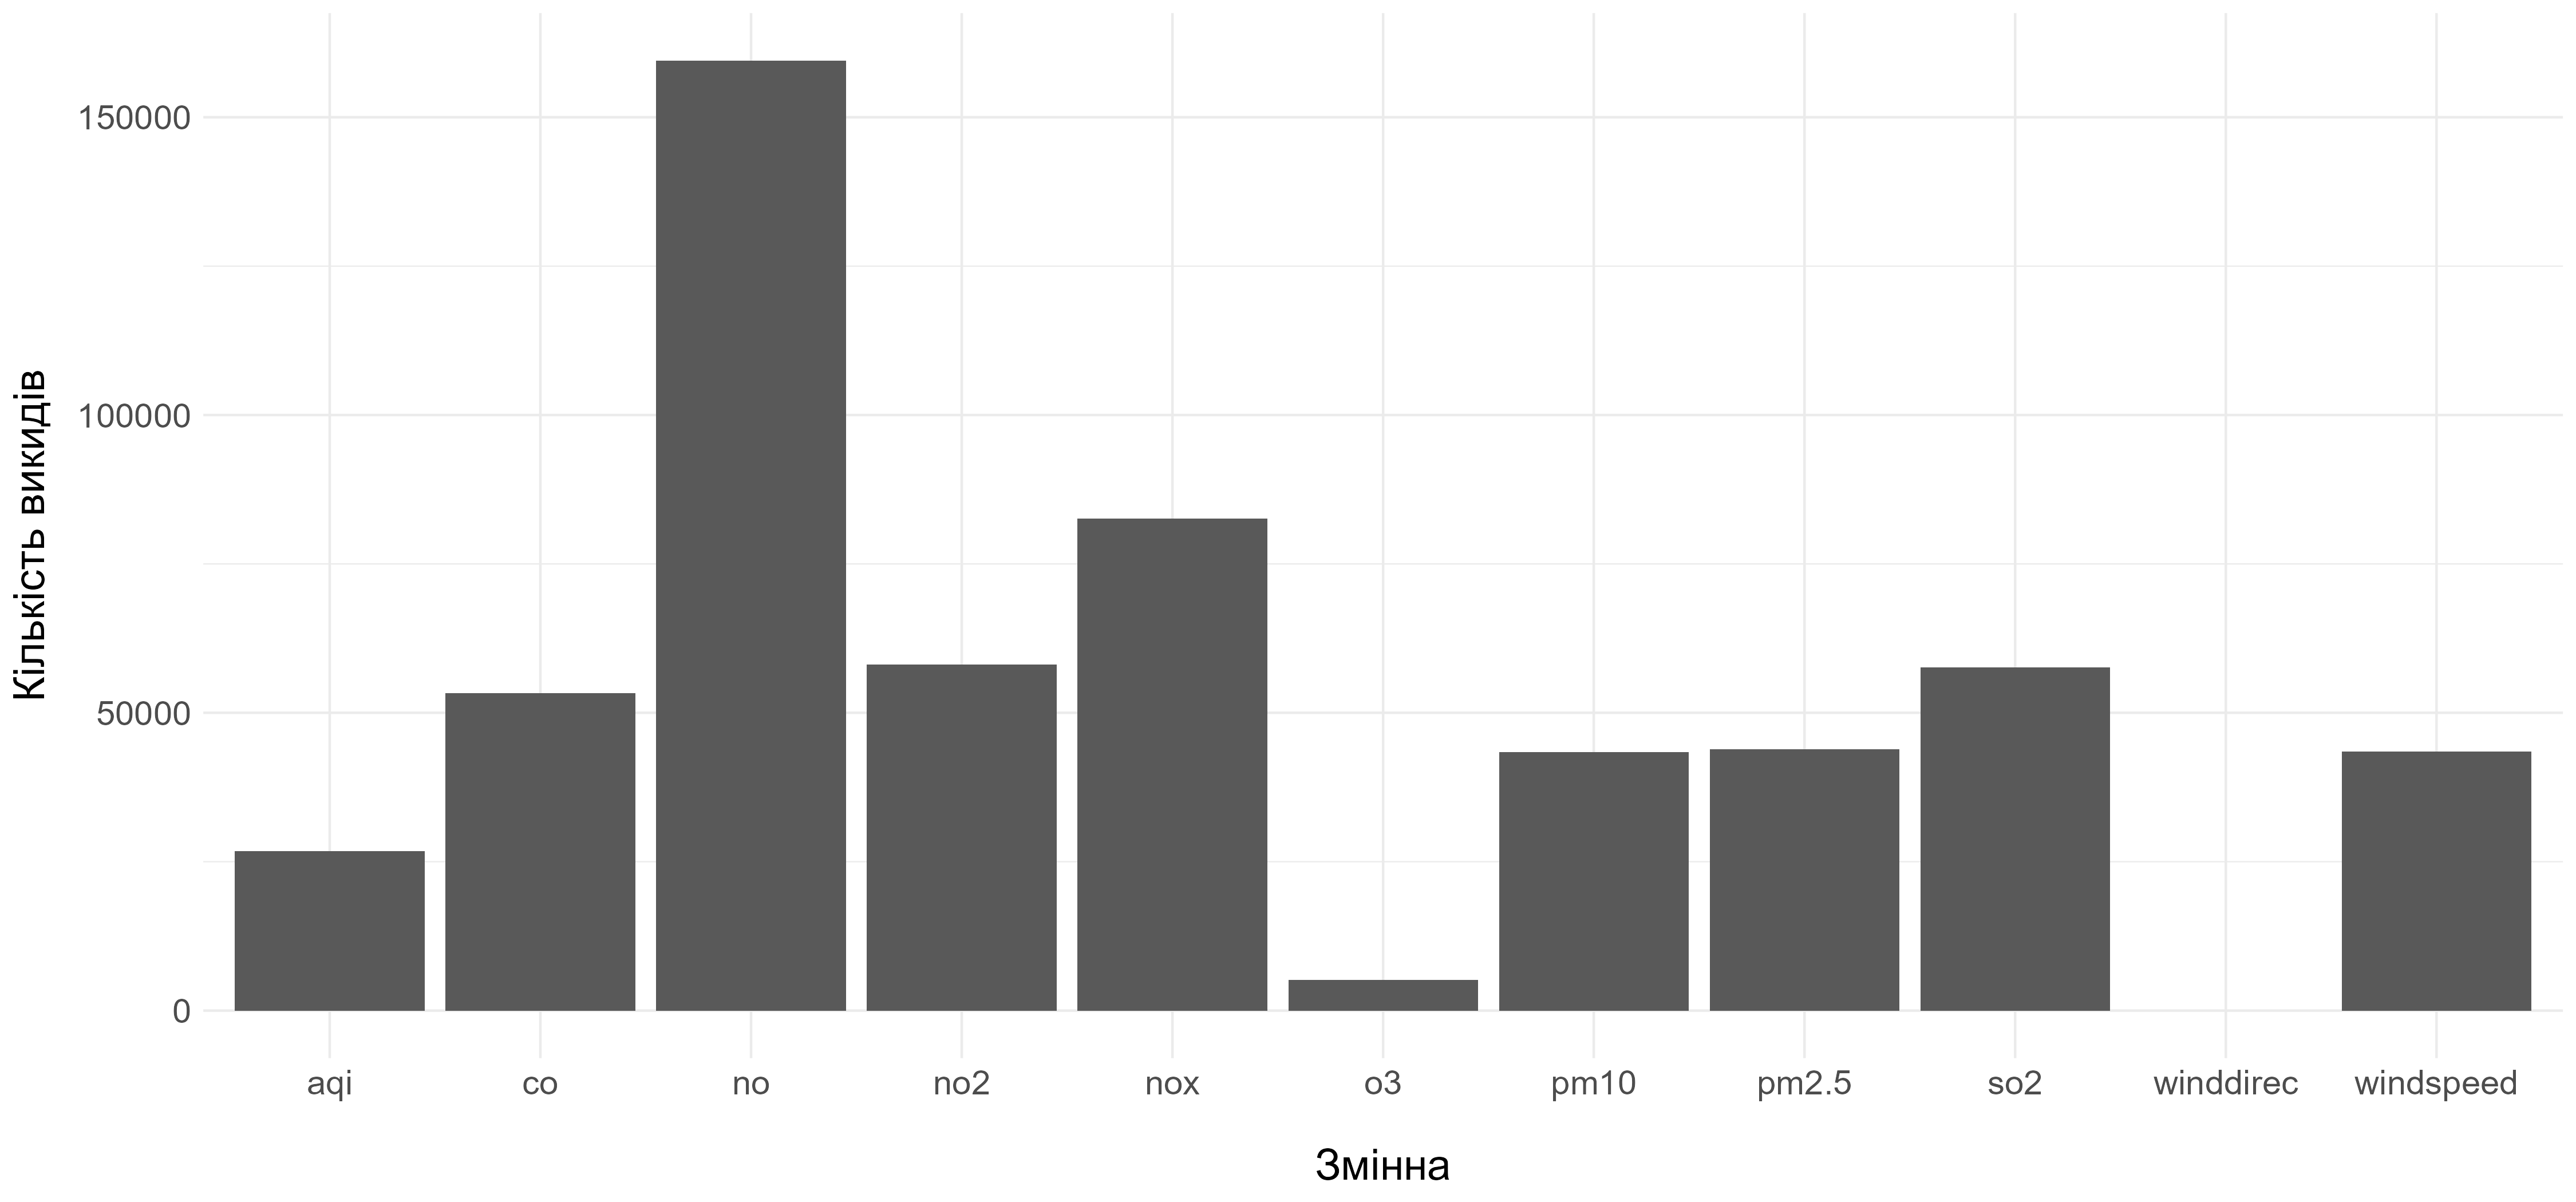
\includegraphics[height=2.7in]{plots/outliers/count-bar.png}

    Гістограма кількості викидів залежно від регіону:

    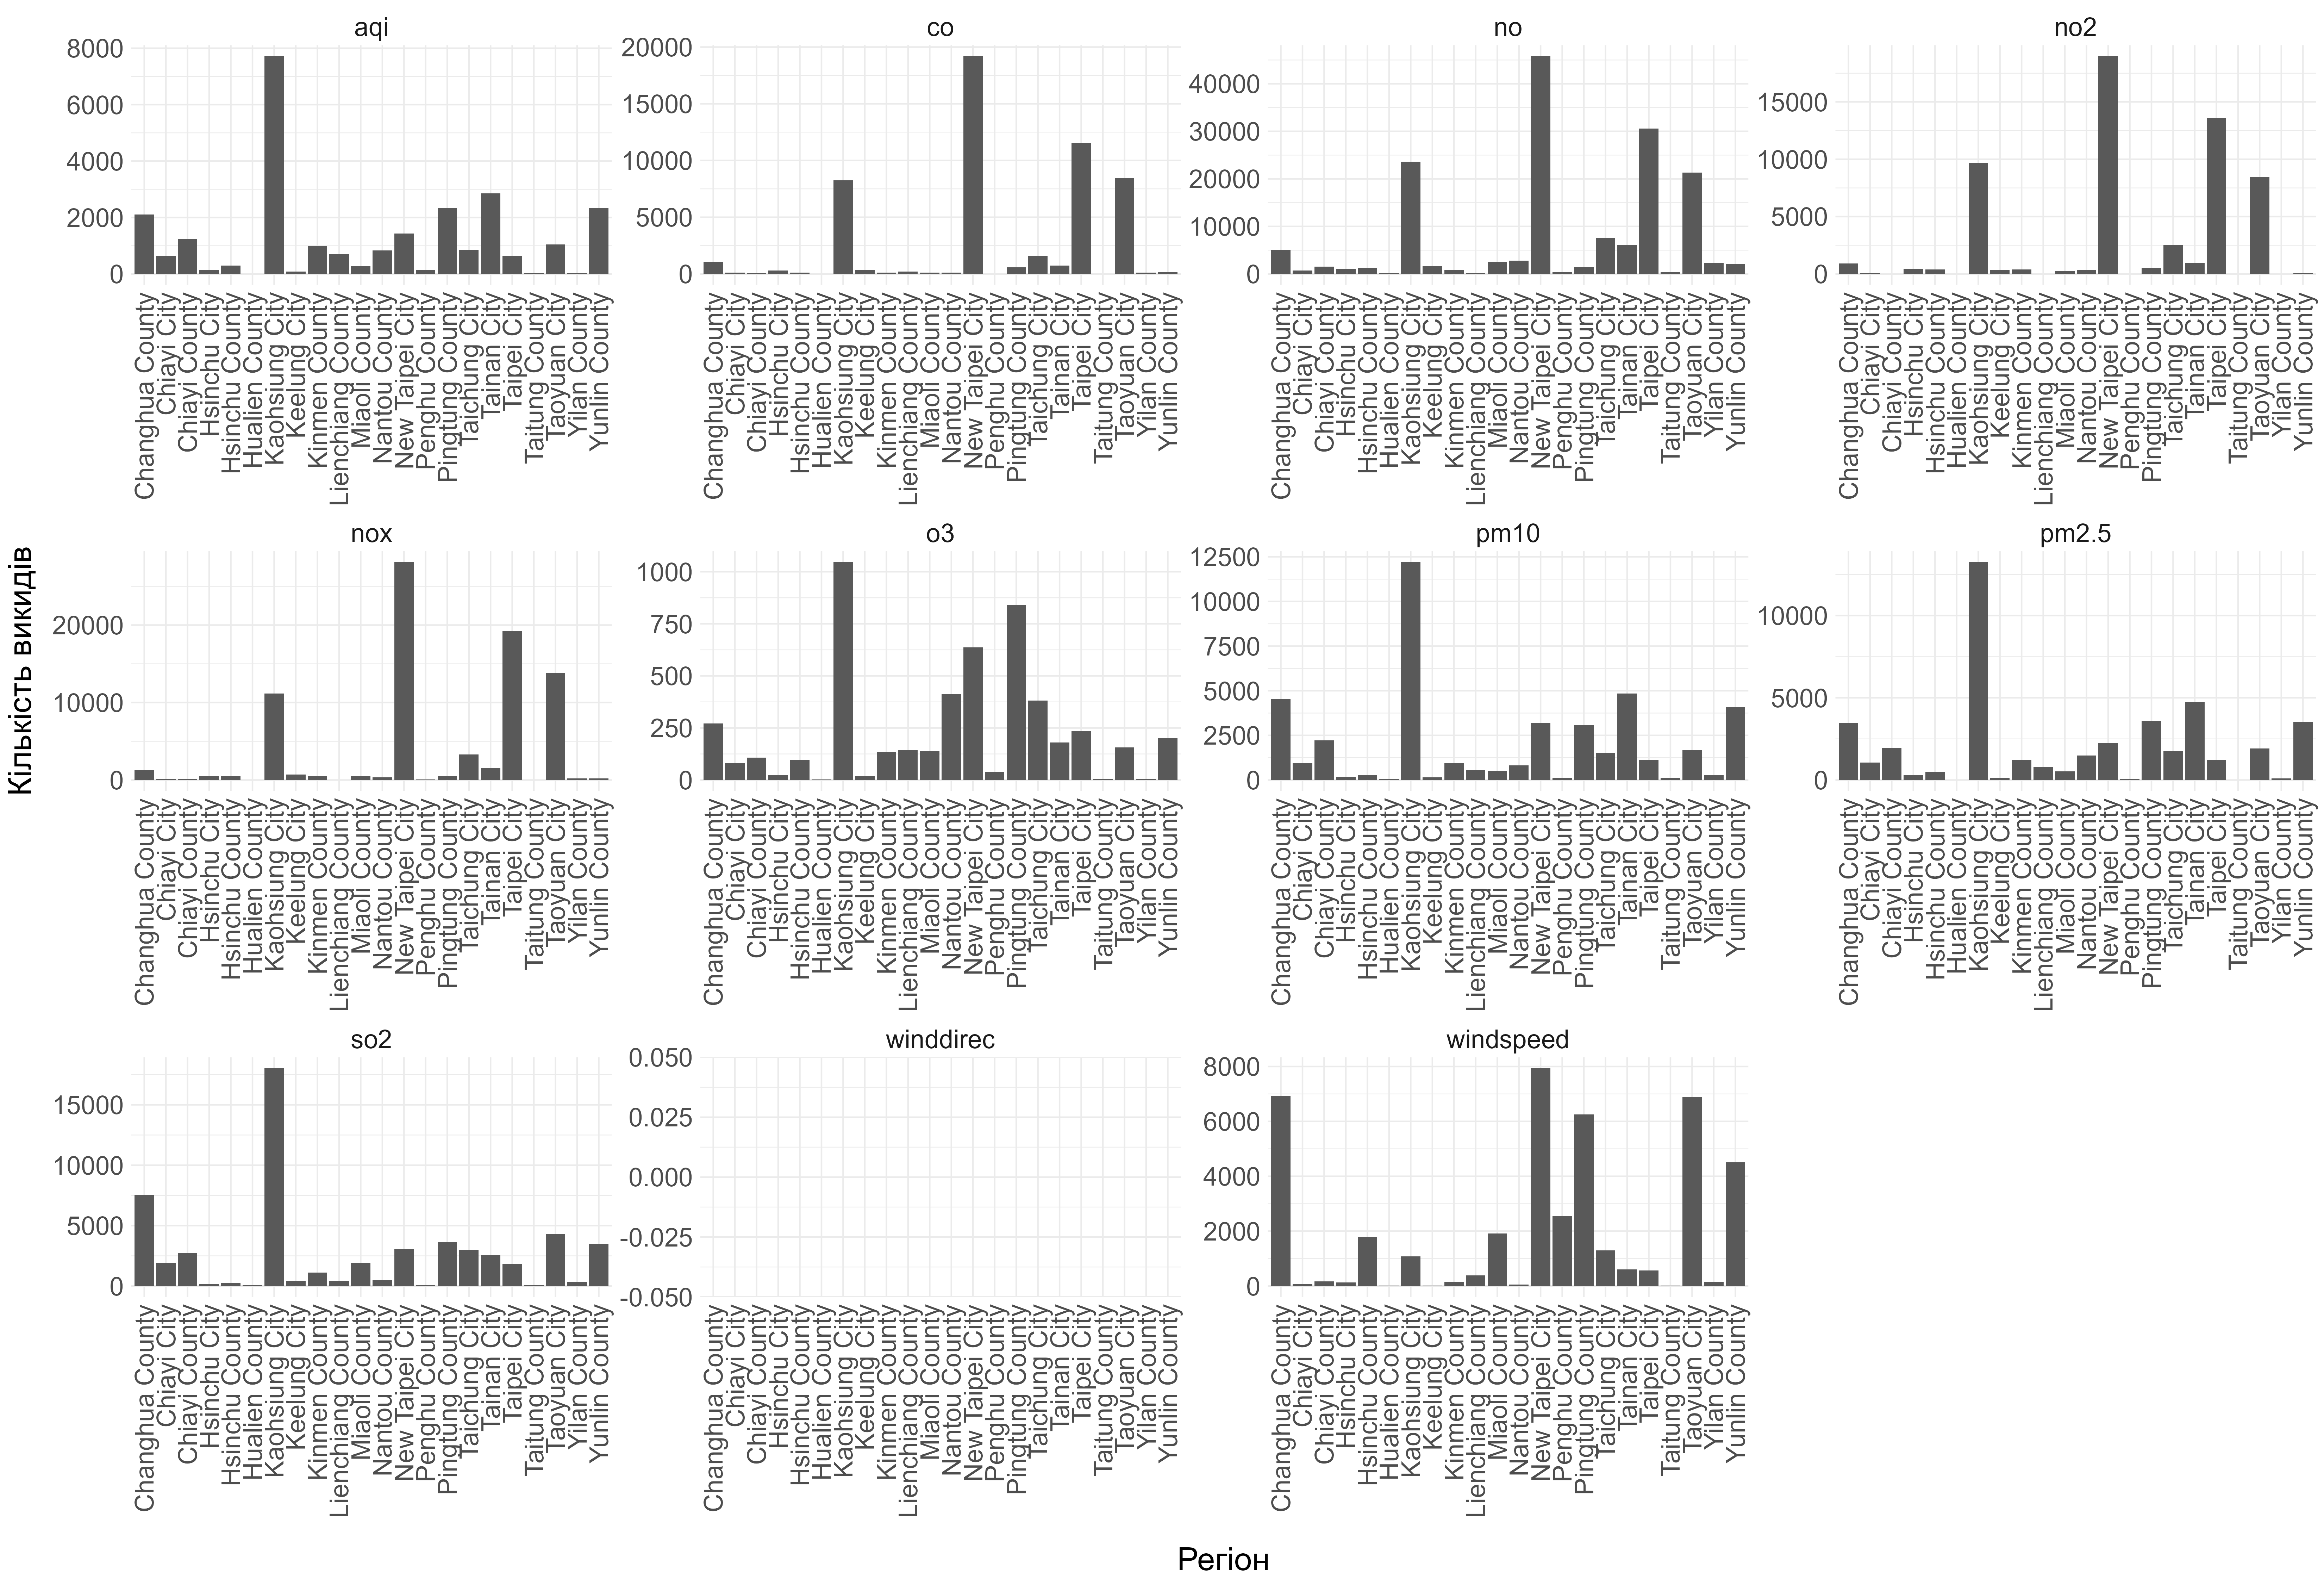
\includegraphics[width=6in]{plots/outliers/count-bar-county.png}

    На гістограмі можна замітити, що кількість викидів не розподілена рівномірно
    по регіонам.

    \pagebreak

    Гістограма розсіювання:

    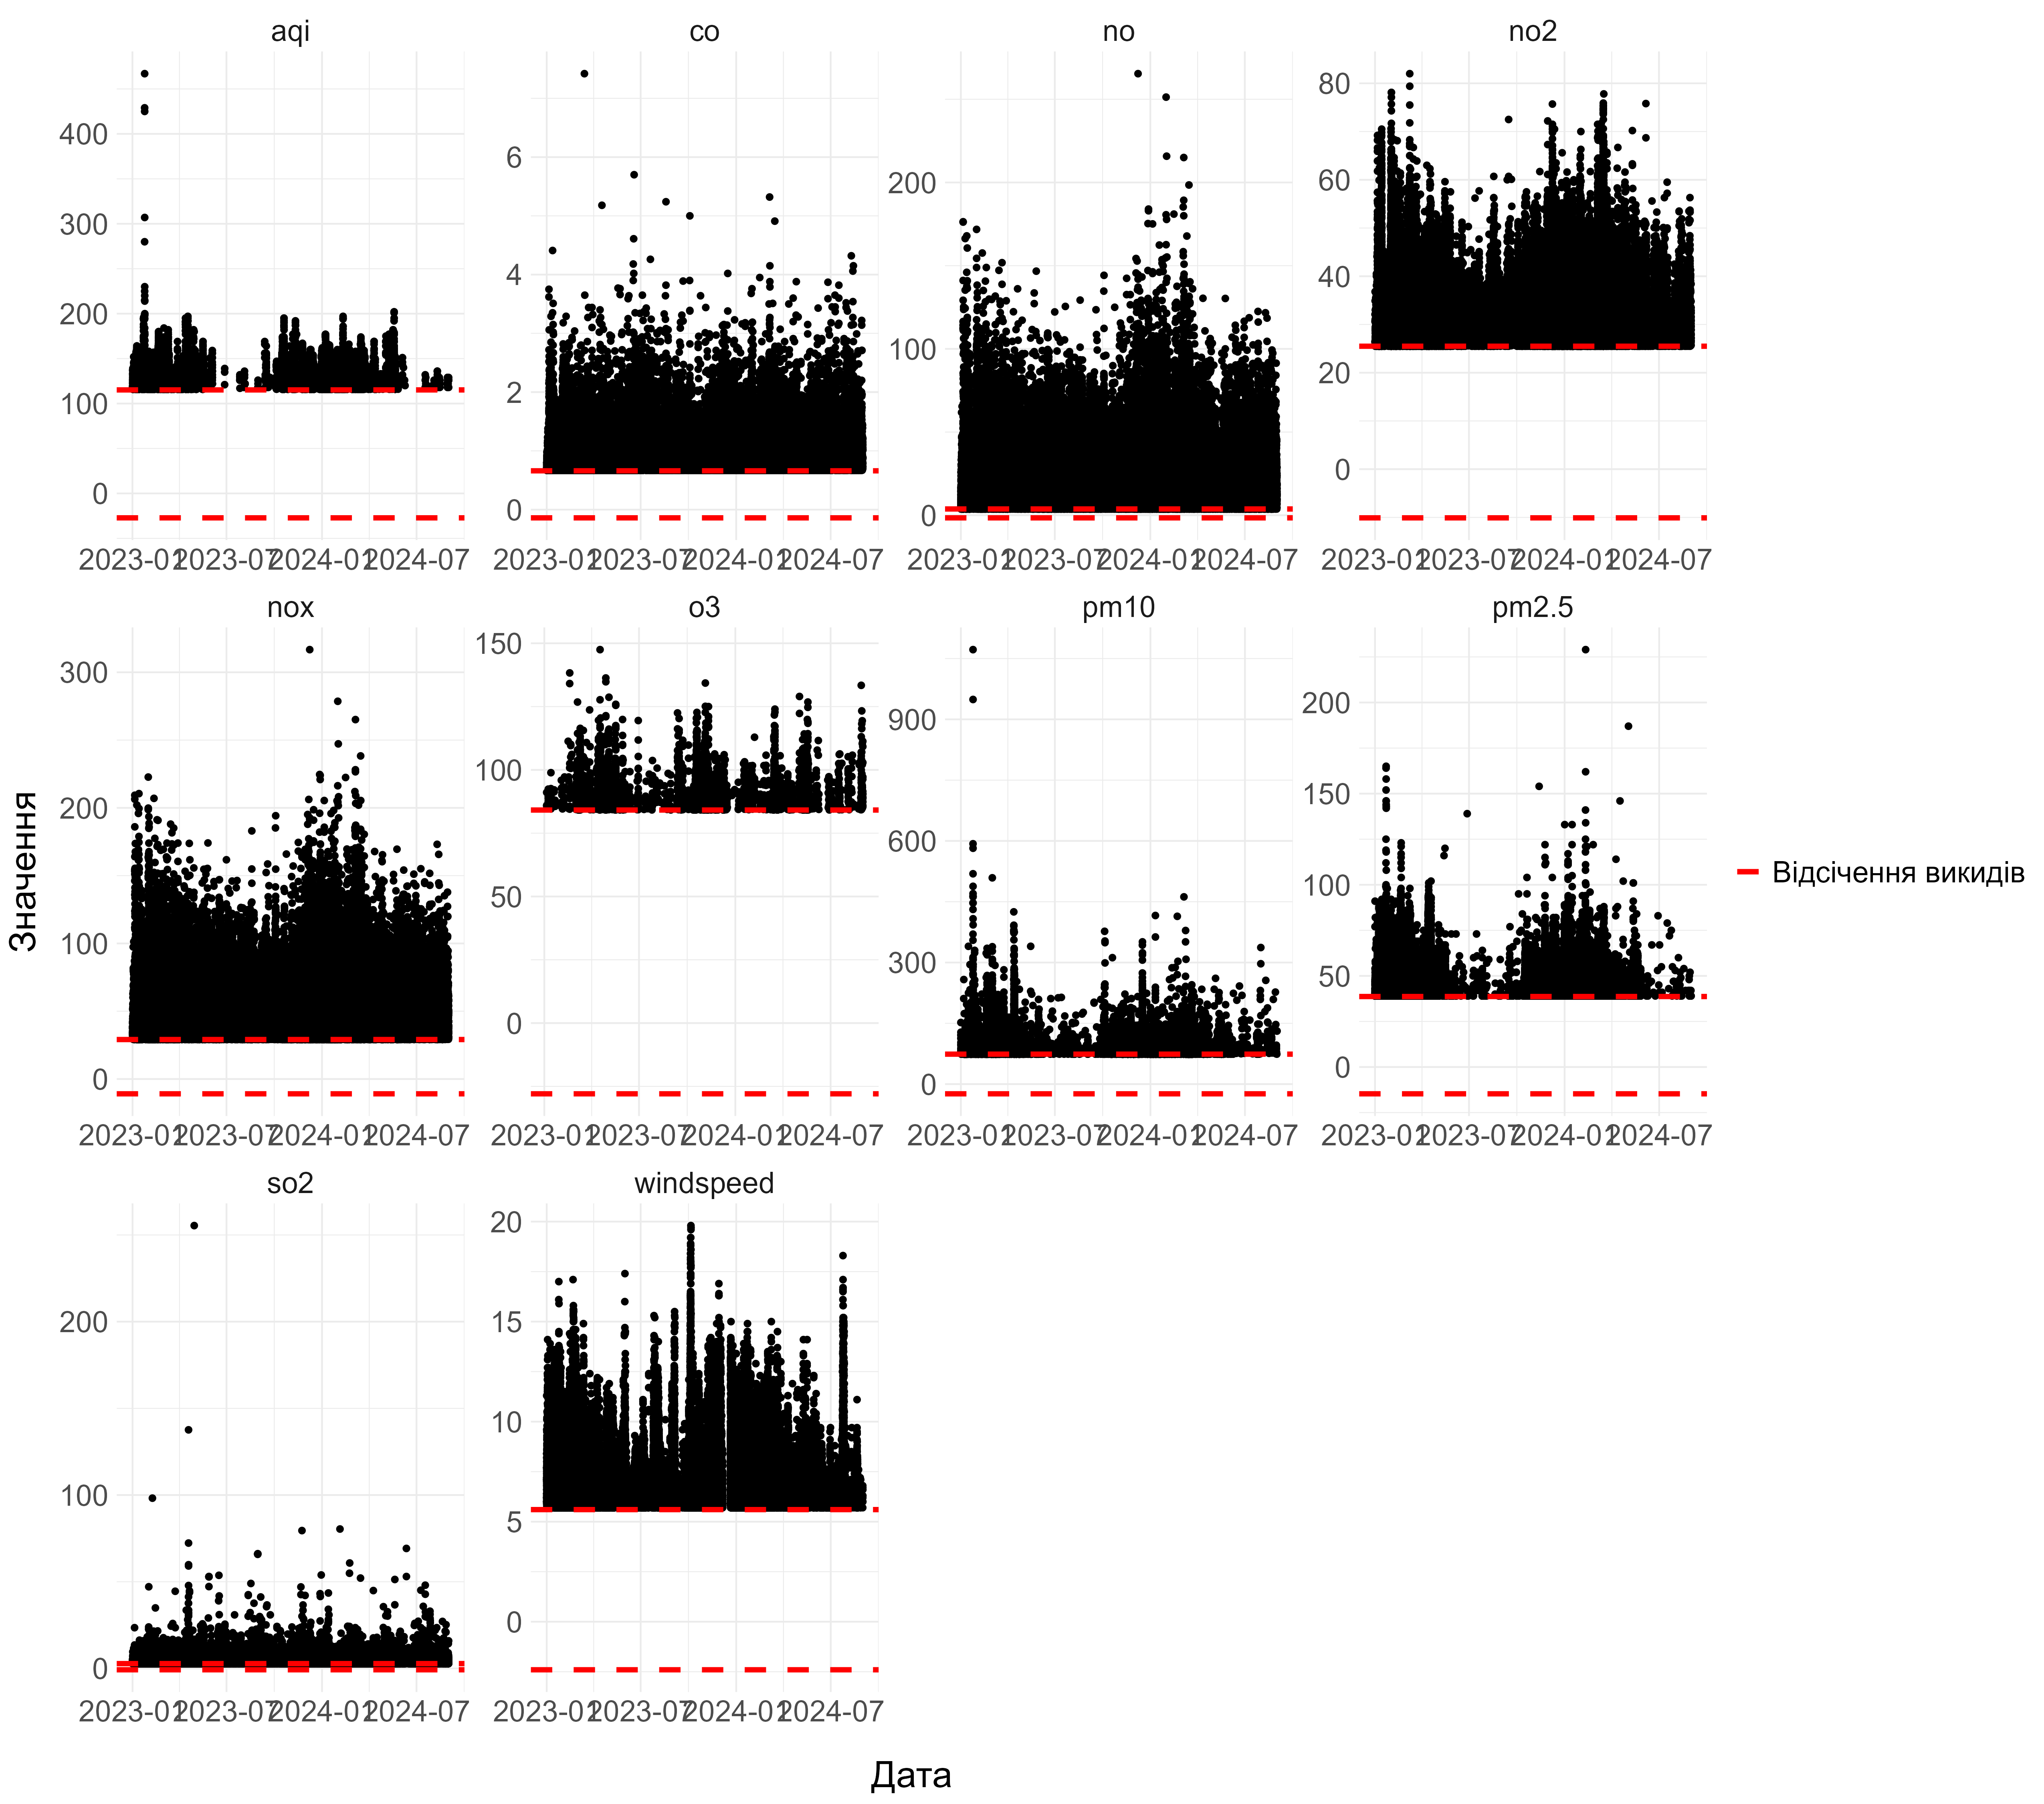
\includegraphics[width=6in]{plots/outliers/scatter.png}

    Червоними лініями позначені проміжки, в яких значення змінної не класифікується
    як викид. На діаграмі розсіювання можна замітити значення, які набагато більші за
    інші викиди. Можна припустити, що вони є помилками датників, які вимірювали якість
    повітря.

    Було прийнято рішення не змінювати значення, або видаляти викиди. Натомість будемо
    використовувати міри вибірок, які більш стійкі до викидів.

    \pagebreak

    \item Розподіли змінних

    Для побудови QQ-графіків, випадковим чином виберемо з датасету 10\,000 рядків.

    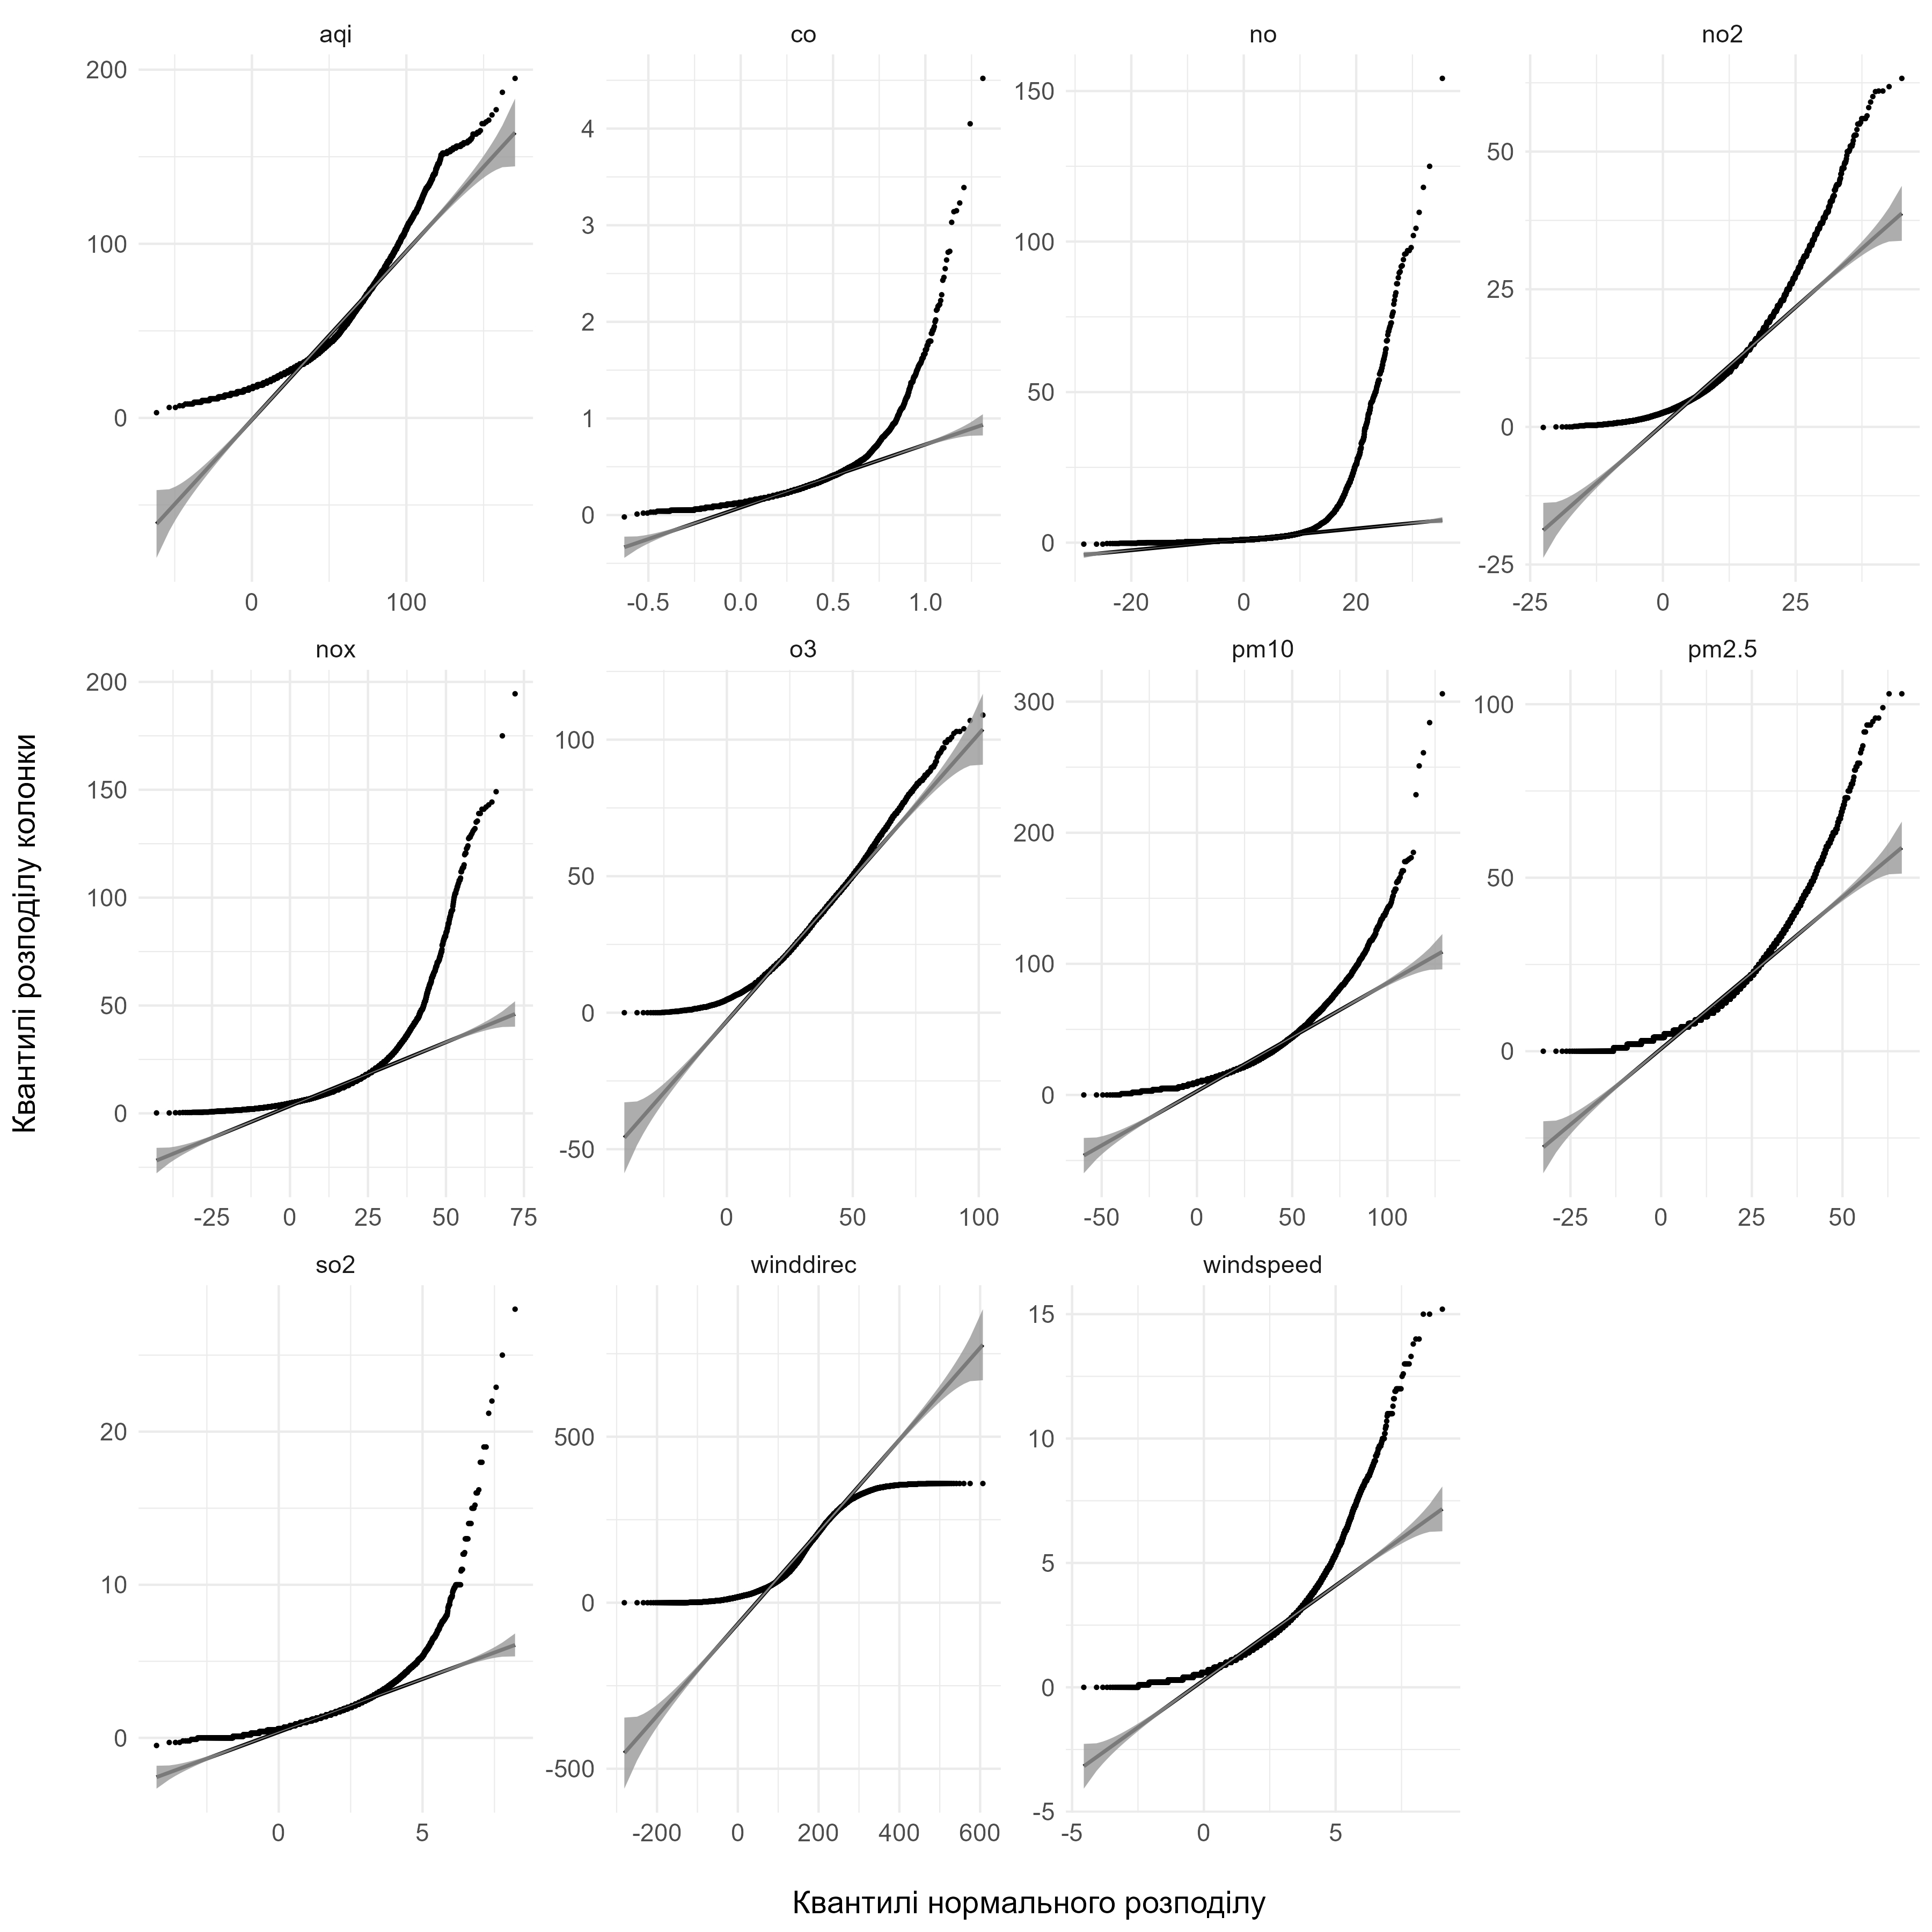
\includegraphics[width=5.5in]{plots/qq_tidy/qq.png}

    \pagebreak

    Розподіл змінних (крім winddirect) ближче до логнормального, ніж нормального:

    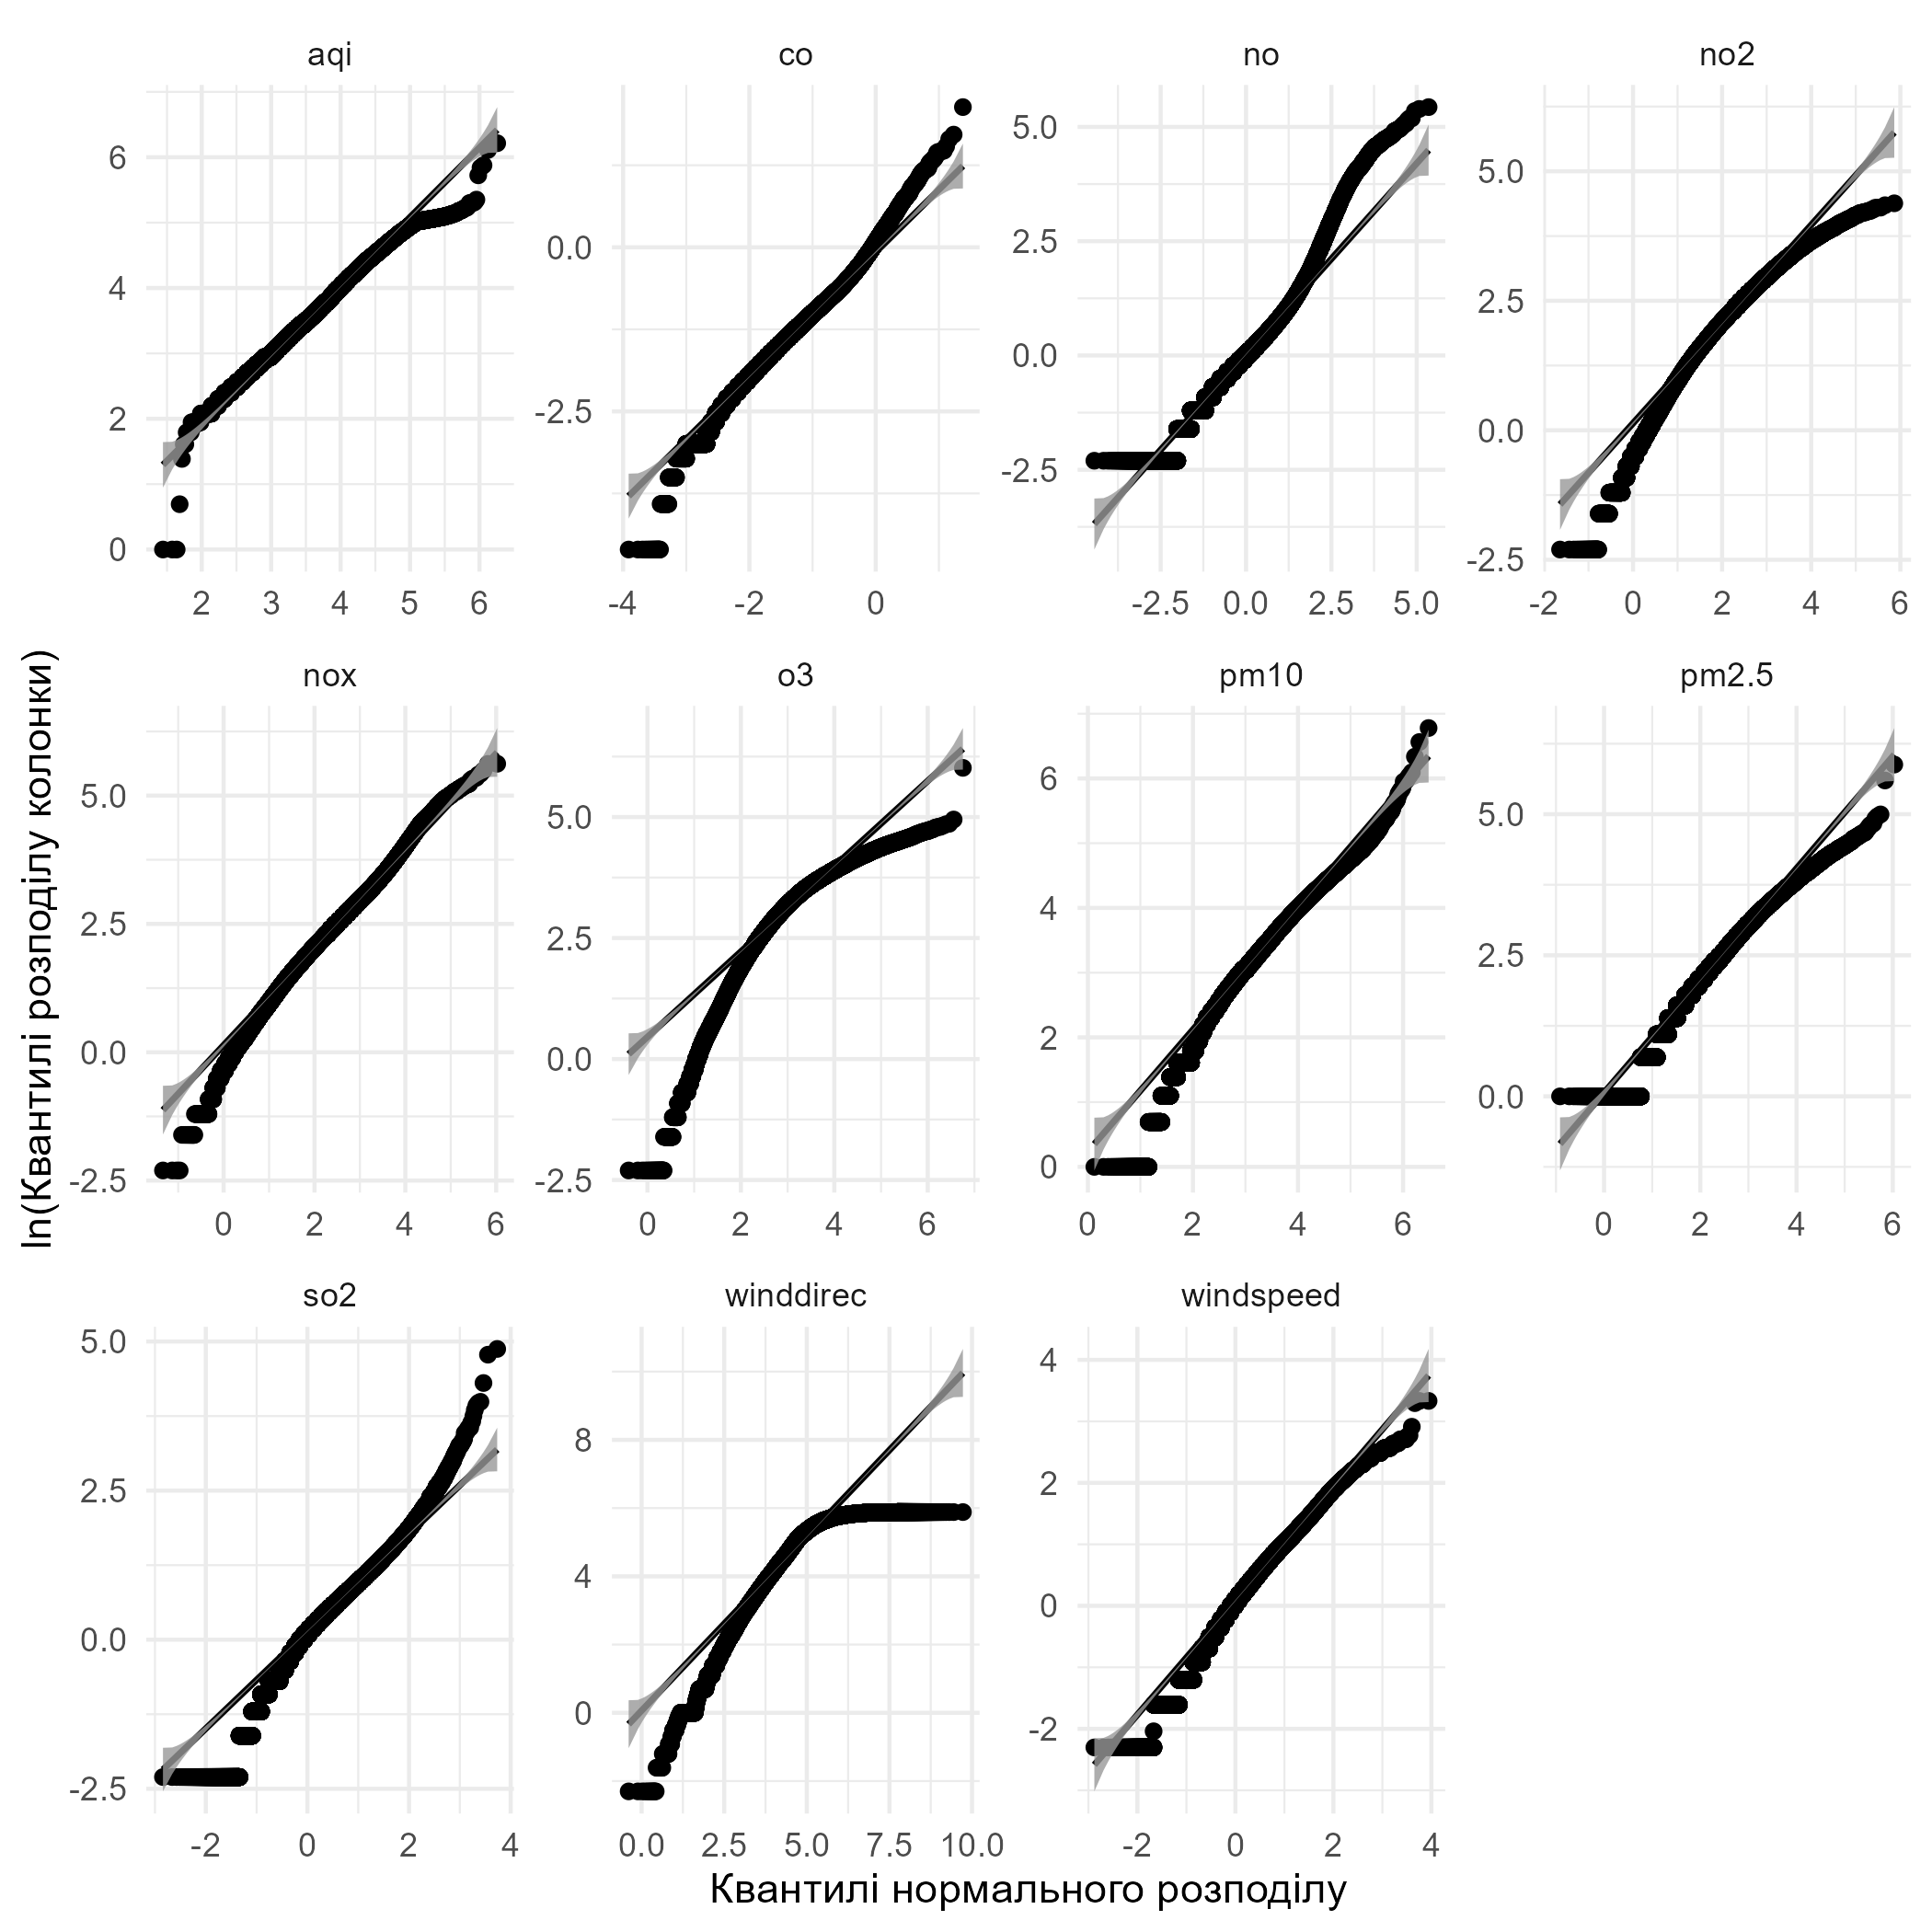
\includegraphics[width=6in]{plots/qq_tidy/qq-log.png}

\end{enumerate}

\end{document}